%!TEX root = ../../csuthesis_main.tex
\chapter{ROV动力学模型参数辨识}
\section{ROV水动力系数辨识方法}

\subsection{最小二乘辨识ROV水动力系数}
最小二乘算法是最早提出的参数估计算法,旨在找到一组未知参数,使得模型输出尽可能贴近实际观测数据。本节利用最小二乘法进行ROV水平面动力学方程的水动力系数辨识,之后将辨识的结果作为RNN深度学习网络参数辨识的参考值。

首先简要介绍最小二乘法。假设未知参数为$X$,状态维度为$n$,一般的传感器或观测手段无法直接测量$X$的具体数值,只能观测$X$各分量的线性组合,假设第$i$个时间步上,$X$满足方程:\begin{equation}
    Z_i=\mathbf{H_i}X+V_i
\end{equation}
式中$Z_i$为$m_i$维向量,$\mathbf{H_i}$和$V_i$分别为第$i$个时间步观测的状态矩阵和测量噪声,假设共进行$r$次观测采样,则有:
\begin{equation}
\left\{\begin{matrix}
Z_1 = \mathbf{H_i}X+V_1\\
Z_2 = \mathbf{H_i}X+V_2\\
\vdots \\
Z_r = \mathbf{H_i}X+V_r\\
\end{matrix}\right. 
\end{equation}

最小二乘算法的核心是使由未知参数的估计值$\hat{X}$计算出的预测值$\hat{Z_i}=\mathbf{H_i}\hat{X}+V_i$和观测值$Z_i$之间的误差平方和最小,定义损失函数为:
\begin{equation}
    J(\hat{X})=\sum_{i=1}^r(Z_i-\mathbf{H_i}\hat{X})^2
\end{equation}
对上述过程中的$\hat{X}$求偏导,当导数为$0$时$J$存在最小值:
\begin{equation}
    \left.\frac{\partial J}{\partial \hat{X}}\right|_{X=\hat{X}}=-2 \mathbf{H}^{T}(Z-\mathbf{H} \hat{X})=0
\end{equation}
则最小二乘法的估计值为:
\begin{equation}
    \hat{X}=(\mathbf{H}^T\mathbf{H})^{-1}\mathbf{H}^TZ
\end{equation}
本节在开始最小二乘辨识之前,先利用高保真仿真平台Gazebo产生Bluerov2在静水中的航行仿真数据,采样频率为$20Hz$,记录电机转速、在全局坐标系下的位置和姿态序列、线速度和角速度序列、线加速度和角加速度序列。在后续辨识过程中,为了模拟实际航行数据,对仿真中的速度序列添加噪声来模拟传感器的采样值,假设速度噪声概率统计满足高斯分布,则采用如下方式添加噪声:
\begin{equation}
\begin{bmatrix}
u_t^*\\
v_t^*\\
w_t^*\\
\end{bmatrix} = \begin{bmatrix}
u_t\\
v_t\\
w_t\\
\end{bmatrix} + randn(0,0.01)
\end{equation}

式中$[u_t^*,v_t^*,w_t^*]^T$表示带有噪声速度数据,$[u_t,v_t,w_t]^T$表示仿真采样速度数据,其中,$randn(0,0.01)\in \mathbb{R}^{3x1}$表示满足均值为0,方差为0.01高斯分布的噪声数据。定义仿真中的真实ROV水动力系数如表\ref{t.real_hydro_coff}所示,ROV基本参数如表\ref{t.rov_base_params}所示。
\begin{table}[htb]
  \centering
  \caption{仿真平台中ROV真实水动力系数}
  \label{t.real_hydro_coff}
  \begin{tabular}{ccccccc}
  \hline
符号 & $X_{\dot{u}}$ & $Y_{\dot{v}}$ & $Z_{\dot{w}}$ & $K_{\dot{p}}$ & $M_{\dot{q}}$ & $N_{\dot{r}}$ \\
\hline
值  & -1.7182         & 0         & -5.468        & 0         & -1.2481         & -0.4006         \\
\hline
\hline
符号 & $X_u$         & $Y_v$         & $Z_w$         & $K_p$         & $M_q$         & $N_r$         \\
\hline
值  & -11.7391         & -20         & -31.8678         & -25         & -44.9085         & -5         \\
\hline
\hline
符号 & $X_{u|u|}$    & $Y_{v|v|}$    & $Z_{w|w|}$    & $K_{p|p|}$    & $M_{q|q|}$    & $N_{r|r|}$    \\
\hline
值  & 0        & 0        & 0        & 0         & 0         & 0 \\  
\hline
\end{tabular}
\end{table}

\begin{table}[htb]
  \centering
  \caption{仿真平台中ROV基本参数}
  \label{t.rov_base_params}
\begin{tabular}{cccccccc}
\hline
符号 & $m$  & $I_x$ & $I_y$ & $I_z$ & $(x_g,y_g,z_g)$ & $\rho_{water}$ & $V$   \\
\hline
值  & 11.2$kg$ & 0.16$kg m^2$  & 0.16$kg m^2$  & 0.16$kg m^2$  & (0,0,0.02$m$)      & 1.028$kg/m^3$        & 11.31$m^3$  \\
\hline
\end{tabular}
\end{table}

\subsection{水平面运动上的最小二乘辨识}
根据上述最小二乘辨识方法,本节首先对运动方程进行解耦,利用ROV水平运动轨迹估计水平面运动中的水动力系数。水平面运动是速度向量被约束到某水平面内和角速度向量保持与水平面垂直的运动形式。在机体坐标系下,由于ROV速度向量$U$始终保持在$oxy$平面内,故冲角$\alpha = 0$,漂角$\beta \ne 0$,又有角速度向量保持与水平面垂直,故线速度中$w=\dot{w}=0$,$p=q=\dot{p}=\dot{q}=0$,将该条件代入动力学分量方程,可以得到ROV在水平面上运动方程各分量的简化形式:


\begin{equation}
\begin{aligned}
X & =(m-X_{\dot{u}})\dot{u}+ (Y_{\dot{v}}-m)vr+(-X_u-X_{u|u|}|u|)u \\
Y & =(m-Y_{\dot{v}})\dot{v}+(m-X_{\dot{u}})ur+(-Y_v-Y_{v|v|}|v|)v \\
N & =(I_z-N_{\dot{r}})\dot{r}+(X_{\dot{u}}-Y_{\dot{v}})vu+(-N_r-N_{r})r 
\end{aligned}
\end{equation}
对前向方程进行整理,可以得到:
\begin{equation}
    \dot{u}=a_1vr+a_2u+a_3u|u|+a_4X
\end{equation}
其中,
\begin{equation}
    a_1=\frac{m-Y_{\dot{v}}}{m-X_{\dot{u}}},a_2=\frac{X_u}{m-X_{\dot{u}}},a_3=\frac{X_{u|u|}}{m-X_{\dot{u}}},a_4=\frac{1}{m-X_{\dot{u}}}
\end{equation}
这四个数为最小二乘法代求系数,按照上述最小二乘算法进行整理,可以得到:
\begin{equation}
    \begin{bmatrix}
    \dot{u}_1 \\
    \dot{u}_2 \\
    \vdots \\
    \dot{u}_T \\
    \end{bmatrix}
    =
    \begin{bmatrix}
    v_1r_1 & u_1 & u_1|u_1| & X_1 \\
    v_2r_2 & u_2 & u_2|u_2| & X_2 \\
    \vdots & \vdots & \vdots & \vdots \\
    v_Tr_T & u_T & u_T|u_T| & X_T \\
    \end{bmatrix}
    \begin{bmatrix}
    a_1 \\
    a_2 \\
    \vdots \\
    a_T \\
    \end{bmatrix}
\end{equation}
式中,$[a_1,a_2,a_3,a_4]^T$为待估计参数,根据上式可以求解出这4个变量,之后先求解$a_4$中的$X_{\dot{u}}$后,可以依次求解出$a_1,a_2,a_3$中的$Y_{\dot{v}},X_u,X_{u|u| }$变量。按照这个方法,ROV侧向运动的动力学方程可整理为:
\begin{equation}
    \dot{v}=b_1ur+b_2v+b_3v|v|+b_4Y
\end{equation}
其中,
\begin{equation}
    b_1=\frac{X_{\dot{u}}-m}{m-Y_{\dot{v}}},b_2=\frac{Y_v}{m-Y_{\dot{v}}},b_3=\frac{Y_{v|v|}}{m-Y_{\dot{v}}},b_4=\frac{1}{m-Y_{\dot{v}}}
\end{equation}

这四个数为最小二乘法代求系数,按照上述最小二乘算法进行处理,可以得到:
\begin{equation}
    \begin{bmatrix}
    \dot{v}_1 \\
    \dot{v}_2 \\
    \vdots \\
    \dot{v}_T \\
    \end{bmatrix}
    =
    \begin{bmatrix}
    u_1r_1 & v_1 & v_1|v_1| & Y_1 \\
    u_2r_2 & v_2 & v_2|v_2| & Y_2 \\
    \vdots & \vdots & \vdots & \vdots \\
    u_Tr_T & v_T & v_T|v_T| & Y_T \\
    \end{bmatrix}
    \begin{bmatrix}
    b_1 \\
    b_2 \\
    \vdots \\
    b_T \\
    \end{bmatrix}
\end{equation}
式中,$[b_1,b_2,b_3,b_4]^T$为待估计参数,根据上式可以求解出这4个变量,之后先求解$b_4$中的$Y_{\dot{v}}$后,可以依次求解出$b_1,b_2,b_3$中的$X_{\dot{u}},Y_v,Y_{v|v| }$变量。

但是考虑到在这两个式子中,$X_{\dot{u}}$与$Y_{\dot{v}}$均得到了两次估计值,为了减小误差,采用两次估计值的平均值作为$X_{\dot{u}}$和$Y_{\dot{v}}$的最终估计值:
\begin{equation}
    \begin{aligned}
        X_{\dot{u}} & =m + \frac{1}{2}\left(\frac{b_1}{b_4}-\frac{1}{a_4}\right)\\
        Y_{\dot{v}}& =m + \frac{1}{2}\left(\frac{a_1}{a_4}-\frac{1}{b_4}\right)
    \end{aligned}
\end{equation}


类似地,可以将ROV水平面回转运动方程整理为:
\begin{equation}
    \dot{r}=c_1vu+c_2r+c_3r|r|+c_4N
\end{equation}

其中,
\begin{equation}
    c_1=\frac{Y_{\dot{v}}-X_{\dot{u}}}{I_z-N_{\dot{r}}},c_2=\frac{N_r}{I_z-N_{\dot{r}}}, c_3=\frac{N_{r|r|}}{I_z-N_{\dot{r}}},c_4=\frac{1}{I_z-N_{\dot{r}}}
\end{equation}
这四个数为最小二乘法代求系数,按照上述最小二乘算法进行处理,可以得到:
\begin{equation}
    \begin{bmatrix}
    \dot{r}_1 \\
    \dot{r}_2 \\
    \vdots \\
    \dot{r}_T \\
    \end{bmatrix}
    =
    \begin{bmatrix}
    v_1u_1 & r_1 & r_1|r_1| & N_1 \\
    v_2u_2 & r_2 & r_2|r_2| & N_2 \\
    \vdots & \vdots & \vdots & \vdots \\
    v_Tu_T & r_T & r_T|r_T| & N_T \\
    \end{bmatrix}
    \begin{bmatrix}
    c_1 \\
    c_2 \\
    \vdots \\
    c_T \\
    \end{bmatrix}
\end{equation}
式中,$[c_1,c_2,c_3,c_4]^T$为待估计参数,根据上式可以求解出这4个变量,其中$c_1$中的$X_{\dot{u}}$和$Y_{\dot{v}}$代入上述由两次取平均得到的最终估计值,并且将$c_1$与$c_4$计算得到的两个$N_{\dot{r}}$估计值的平均值作为$N_{\dot{r}}$的最终估计值,之后可以依次求解出$c_2,c_3$中的$N_r,N_{r|r|}$变量。$N_{\dot{r}}$的最终估计值为:
\begin{equation}
    N_{\dot{r}} = I_z - \frac{1}{2}(\frac{1}{c_4} + \frac{Y_{\dot{v}}-X_{\dot{u}}}{c_1})
\end{equation}

水平面运动的最小二乘辨识结果如表\ref{t._hydro_coff_ident_horizon}所示。

\begin{table}[htb]
  \centering
  \caption{ROV水平面运动水动力系数辨识结果}
  \label{t._hydro_coff_ident_horizon}
  \begin{tabular}{ccccccc}
  \hline
符号 & $X_{\dot{u}}$ & $Y_{\dot{v}}$ & $N_{\dot{r}}$ \\
\hline
辨识值  & -1.98          & -0.2410          & -0.6560         \\
\hline
\hline
符号 & $X_u$         & $Y_v$            & $N_r$         \\
\hline
辨识值  & -9.3790         & -4.180            & -18.780         \\
\hline
\hline
符号 & $X_{u|u|}$    & $Y_{v|v|}$     & $N_{r|r|}$    \\
\hline
辨识值  & -0.78        & -4.77            & -1.73 \\  
\hline
\end{tabular}
\end{table}

通过辨识出的水动力系数计算动力学模型的前向推导,结果如图\ref{f.dynamic_forward_identified}所示。该曲线图将预测数据与高保真仿真平台下的仿真数据进行对比,两支曲线均是对于相同水下机器人,在相同水环境和相同推进器驱动力下运行,通过计算误差可以发现,$u,v,r$误差范围保持在真值的$1\%$之内,并且辨识得到的运动数据误差累计效应表现不显著,能够有效还原BlueROV2的运动数据。
\begin{figure}[hbt]
    \centering
    \includegraphics[width=\linewidth]{images/chapter3/3.1 水平面最小二乘辨识.jpg}
    \caption{采用水动力系数估计值的水平面前向动力学推导}
    \label{f.dynamic_forward_identified}
\end{figure}
\subsection{竖直面运动的最小二乘辨识}

通过上述方法,本文在高保真仿真平台内使用控制器控制BlueROV2产生一组竖直面内的运动,竖直面运动是速度向量被约束到竖直面内和角速度向量保持与竖直面垂直的运动形式,在机体坐标系下,满足$v=u=\dot{v}=\dot{u}=0$,$r=\dot{r}=0$,将该条件代入动力学分量方程后依照上述方法转换成最小二乘形式,可以辨识出ROV系统水动力系数如表\ref{t._hydro_coff_ident_vertical}所示。

通过辨识出的水动力系数计算动力学模型的前向推导,结果如图\ref{f.dynamic_forward_identified_vertical}所示。将预测数据与高保真仿真平台下的仿真数据进行对比,两支曲线均是对于相同水下机器人,在相同水环境和相同推进器驱动力下运行,通过计算误差可以发现,$w,p,q$误差波动较大,表现不如水平面运动下的最小二乘辨识,但是也能较好拟合实际轨迹运动数据。

\begin{table}[htb]
  \centering
  \caption{ROV竖直面运动水动力系数辨识结果}
  \label{t._hydro_coff_ident_vertical}
  \begin{tabular}{ccccccc}
  \hline
符号 & $Z_{\dot{w}}$ & $K_{\dot{p}}$ & $M_{\dot{q}}$ \\
\hline
辨识值  & -14.57   & -0.12  &   -3.45         \\
\hline
\hline
符号 & $Z_w$         & $K_p$            & $M_q$         \\
\hline
辨识值  & -25.89         & -30.40       & -45.90         \\
\hline
\hline
符号 & $Z_{w|w|}$    & $K_{p|p|}$     & $M_{q|q|}$    \\
\hline
辨识值  & -3.21        & -5.21        & -0.23 \\  
\hline
\end{tabular}
\end{table}

\begin{figure}[hbt]
    \centering
    \includegraphics[width=\linewidth]{images/chapter3/竖直面最小二乘辨识.png}
    \caption{采用水动力系数估计值的竖直面前向动力学推导}
    \label{f.dynamic_forward_identified_vertical}
\end{figure}

\subsection{六自由度运动的最小二乘辨识}
本节对六个自由度的机器人运动过程,采用最小二乘方法辨识水动力系数。对于完整的动力学分量形式,可以将其整理为最小二乘法的形式。

定义在第$i$个时间步下,有矩阵:
\begin{equation}
    F_i
    =\left[
    \begin{matrix}
        X_i-m\dot{u}_i-(w_iq_i-v_ir_i)m\\
        Y_i-m\dot{v}_i-(u_ir_i-w_ip_i)m\\
        Z_i-m\dot{w}_i-(v_ip_i-u_iq_i)m\\
        K_i-I_x\dot{p}_i-q_ir_i(J_z-J_y)\\
        M_i-I_y\dot{q}_i-r_ip_i(J_x-J_z)\\
        N_i-I_z\dot{r}_i-p_iq_i(J_y-J_x)\\
    \end{matrix}
\right]
\end{equation}


\begin{equation}
    \mathbf{A_1} = 
    \left[
    \small
    \begin{matrix}
        -\dot{u}_i & v_ir_i & -w_iq_i & 0 & 0 & 0 \\
        -u_ir_i & -\dot{v}_i & w_ip_i & 0 & 0 & 0 \\
        u_iq_i & -v_ip_i & -\dot{w}_i & 0 & 0 & 0 \\
        0 & v_iw_i & -v_iw_i & -\dot{p}_i & q_ir_i & -q_ir_i \\
        -u_iw_i & 0 & u_iw_i & -r_ip_i & -\dot{q}_i & r_ip_i \\
        u_iv_i & -u_iv_i & 0 & p_iq_i & -p_iq_i & -\dot{r}_i \\
    \end{matrix}
    \right]
\end{equation}
\begin{equation}
    \mathbf{A_2} = -diag([u_i,v_i,w_i,p_i,q_i,r_i])
\end{equation}
\begin{equation}
    \mathbf{A_3} = -diag([u_i|u_i|,v_i|v_i|,w_i|w_i|,p_i|p_i|,q_i|q_i|,r_i|r_i|]) 
\end{equation}
\begin{equation}
    \mathbf{A}=[\mathbf{A_1}, \mathbf{A_2}, \mathbf{A_3}] 
\end{equation}
\begin{equation}
    \Theta_1 = [X_{\dot{u}}, Y_{\dot{v}}, Z_{\dot{w}}, K_{\dot{p}}, M_{\dot{u}}, N_{\dot{r}}]^T
\end{equation}
\begin{equation}
    \Theta_2 = [X_u, Y_v, Z_w, K_p, M_q, N_r]
\end{equation}
\begin{equation}
    \Theta_3 = [X_{u|u|}, Y_{v|v|}, Z_{w|w|}, K_{p|p|}, M_{q|q|}, N_{r|r|}]
\end{equation}
\begin{equation}
    \Theta = [ \Theta_1, \Theta_2, \Theta_3 ]
\end{equation}
\begin{equation}
    \boldsymbol{F} = \boldsymbol{A}\boldsymbol{\Theta}
\end{equation}

通过该组实验,发现直接对六自由度运动过程进行辨识,会导致ROV动力学方程的前向推导发散,经过模型对比分析,动力学模型的发散应该是由于六自由度联动辨识导致不适定或误差放大。最小二乘法要求回归矩阵 $A$ 的列向量彼此线性独立,才能稳定解出参数,但实际运行过程中可能各个自由度之间存在强耦合关系,某些列之间高度相关,使得最小二乘结果不稳定且导致模型发散。

\section{扩展卡尔曼滤波器辨识水动力系数}

接下来,本研究采用扩展卡尔曼滤波器(EKF)从六自由度运动过程辨识水动力系数, EKF辨识算法是在经典线性卡尔曼滤波方法的基础上发展而来的,其显著的优势在于基于状态空间局部线性化点(Kalman滤波值)和测量局部线性化点附近的泰勒级数展开对ROV非线性动力学系统模型进行局部线性化,适用于动态非线性模型。

一般地,离散水动力辨识方法可视为有限输入的灰箱结构,该结构迭代地对ROV动力学模型进行参数估计。由于待定系数的状态空间维数与输入输出的状态空间维数之间不相容,18个水动力线性阻尼系数将无法直接辨识,需要将其作为额外的状态变量$\Theta $增广到EKF算法的状态空间转换模型中。

\subsection{扩展卡尔曼滤波器算法简介}

为引入扩展卡尔曼滤波器,首先定义增广状态向量$\hat{X}_{k-1|k-1}$,满足
\begin{equation}
    \hat{X}_{k-1|k-1} = [u,v,w,p,q,r,\phi, \theta, \psi, \Theta]^T_{k-1|k-1}  
\end{equation}
定义由传感器测量得到的测量向量$Z_k$,满足
\begin{equation}
    Z_k=[u,v,w,p,q,r,\phi,\theta,\psi]^T
\end{equation}
由此,系统状态转移方程可以被定义为:
\begin{equation}
    X_k=f_a\left(\hat{X}_{k-1|k-1}, \Theta_{k-1}, u_{k-1}, k-1\right) + \Phi_{k|k-1}\left(X_{k-1}-\hat{X}_{k-1|k-1}\right) + \gamma_{k|k-1}W_{k-1}
\end{equation}

系统测量方程被定义为:
\begin{equation}
    Z_k = h\left(\hat{X}_{k|k-1},k\right)+H_k\left(X_k-\hat{X}_{k|k-1}\right)+M_kV_k
\end{equation}

其中,

$f_a(\cdot)$为增广动力学模型方程;

$h(\cdot)$为系统测量方程;

$\Phi_{k|k-1}=\{\partial f_a(\hat{X}_{k-1|k-1}, \Theta_{k-1}, u_{k-1}, k-1)/\partial X \}|_{\hat{X}_{k-1|k-1}}$为第$k$时间步下的先验增广状态空间转移雅各比矩阵;

$\gamma_{k|k-1}=\{\partial f_a(\hat{X}_{k-1|k-1}, \Theta_{k-1}, u_{k-1}, k-1)/\partial W\}|_{\hat{X}_{k-1|k-1}}$为第$k$时间步下的先验系统过程噪声雅各比矩阵;

$H_k=\{\partial h(\hat{X}_{k|k-1},k)/\partial X\}|_{\hat{X}_{k-1|k-1}}$为第$k$时间步下的系统测量雅各比矩阵;

$M_k=\{\partial h(\hat{X}_{k|k-1},k)/\partial V\}|_{\hat{X}_{k-1|k-1}}$为第$k$时间步下的系统测量噪声雅各比矩阵。

这样,类似于线性卡尔曼滤波方法,ROV的扩展准线性系统模型可以通过离散EKF算法依次经过时间更新阶段和测量更新阶段从式中辨识出来。时间更新阶段满足:

\begin{equation}
    \begin{aligned}
            \hat{X}_{k|k-1} & =f_a\left(\hat{X}_{k-1|k-1}, \Theta_{k-1}, u_{k-1}, k-1\right) \\
            \mathbf{P}_{k|k-1} & = E\left[\tilde{X}_{k|k-1},\tilde{X}^T_{k|k-1} \right] \\ 
              & =E\left[(\Phi_{k|k-1}\tilde{X}_{k-1|k-1} + \gamma_{k|k-1}W_{k-1})(\Phi_{k|k-1}\tilde{X}_{k-1|k-1} + \gamma_{k|k-1}W_{k-1})^T\right] \\
              & =\Phi_{k|k-1}\mathbf{P}_{k-1|k-1}\Phi_{k|k-1}^T + \gamma_{k|k-1}Q_{k-1}\gamma_{k|k-1}^T
    \end{aligned}
\end{equation}

测量更新阶段满足:
\begin{equation}
\begin{aligned}
        \varepsilon_{k} & =Z_k - H_k\hat{X}_{k|k-1} \\
                        & = H_k\tilde{X}_{k|k-1} + M_kV_k \\
        E\left[\varepsilon_k, \varepsilon_k^T\right] & = H_kP_{k|k-1}H_k^T + M_kR_kM_k^T \\
        K_k  & = E\left[X_k, \varepsilon_k^T\right]E\left[\varepsilon_k, \varepsilon_k^T\right]^{-1} \\
        & =E\left[\left(\hat{X}_{k|k-1}+\tilde{X}_{k|k-1}\right)\left(H_k\tilde{X}_{k|k-1} + M_kV_k\right)^T\right](H_kP_{k|k-1}H_k^T + M_kR_kM_k^T)^{-1}\\
        & =(P_{k|k-1}H_k^T)(H_kP_{k|k-1}H_k^T + M_kR_kM_k^T)^{-1} \\
        \hat{X}_{k|k} & =\hat{X}_{k|k-1}+K_k\varepsilon_k \\
        & = \hat{X}_{k|k-1} + K_k(Z_k-H_k\hat{X}_{k|k-1}) \\
        P_{k|k} & =E\left[\tilde{X}_{k|k}\tilde{X}_{k|k}^T\right] \\
        & = (T_n - K_kH_k)P_{k|k-1} 
\end{aligned}
\end{equation}
其中,

$P_{k|k-1}$为第$k$时间步下,先验误差协方差矩阵的预测估计值;

$P_{k-1|k-1}$为后验估计值误差的协方差矩阵;

$P_{k|k}$为后验误差协方差矩阵的更新估计值;

$E[\cdot]$为期望计算函数;

$\tilde{X}_{k|k-1}$为增广状态向量的先验卡尔曼滤波误差;

$\tilde{X}_{k-1|k-1}$为第$k-1$时间步下,增广状态向量的后验卡尔曼滤波误差;

$\hat{X}_{k|k}$为后验增广状态向量的更新估计值;

$\tilde{X}_{k|k}$为增广状态向量的后验滤波误差;

$Q_{k-1}$为第$k-1$时间步下,系统过程噪声协方差矩阵;

$R_{k-1}$为第$k-1$时间步下,系统测量噪声协方差矩阵;

$\varepsilon_k$为第$k$时间步下,系统测量残差向量;

$K_k$为卡尔曼更新增益矩阵;

$I_n$为$n$阶单位矩阵。

在标准时域离散EKF辨识算法的每个单位时间步中,测量更新算法将通过计算卡尔曼滤波更新增益,更新一组后验增广状态向量与相对应的后验误差协方差矩阵,通过增广状态向量的更新得到待辨识参数的估计值。

\subsection{扩展卡尔曼滤波器辨识流程}

本文基于MATLAB/Simulink仿真工具,构建了扩展卡尔曼滤波器在BlueROV2上的仿真框架\cite{munguiaEKFBasedParameterIdentification2019},仿真框架如图\ref{f.EKF_ident_frame}所示。BlueROV2在航行过程中,其传感器数据经过导航系统进行状态估计。控制系统根据估计的状态产生控制指令驱动执行器。同时,控制指令 $\symbf{u}$ 和导航系统的观测数据 $\symbf{z}$ 被送到一个独立的EKF参数辨识模块。该模块利用这些实时数据来估计和更新水下机器人的数学模型参数 $\hat{\symbf{x}}$。

\begin{figure}[hbt]
    \centering
    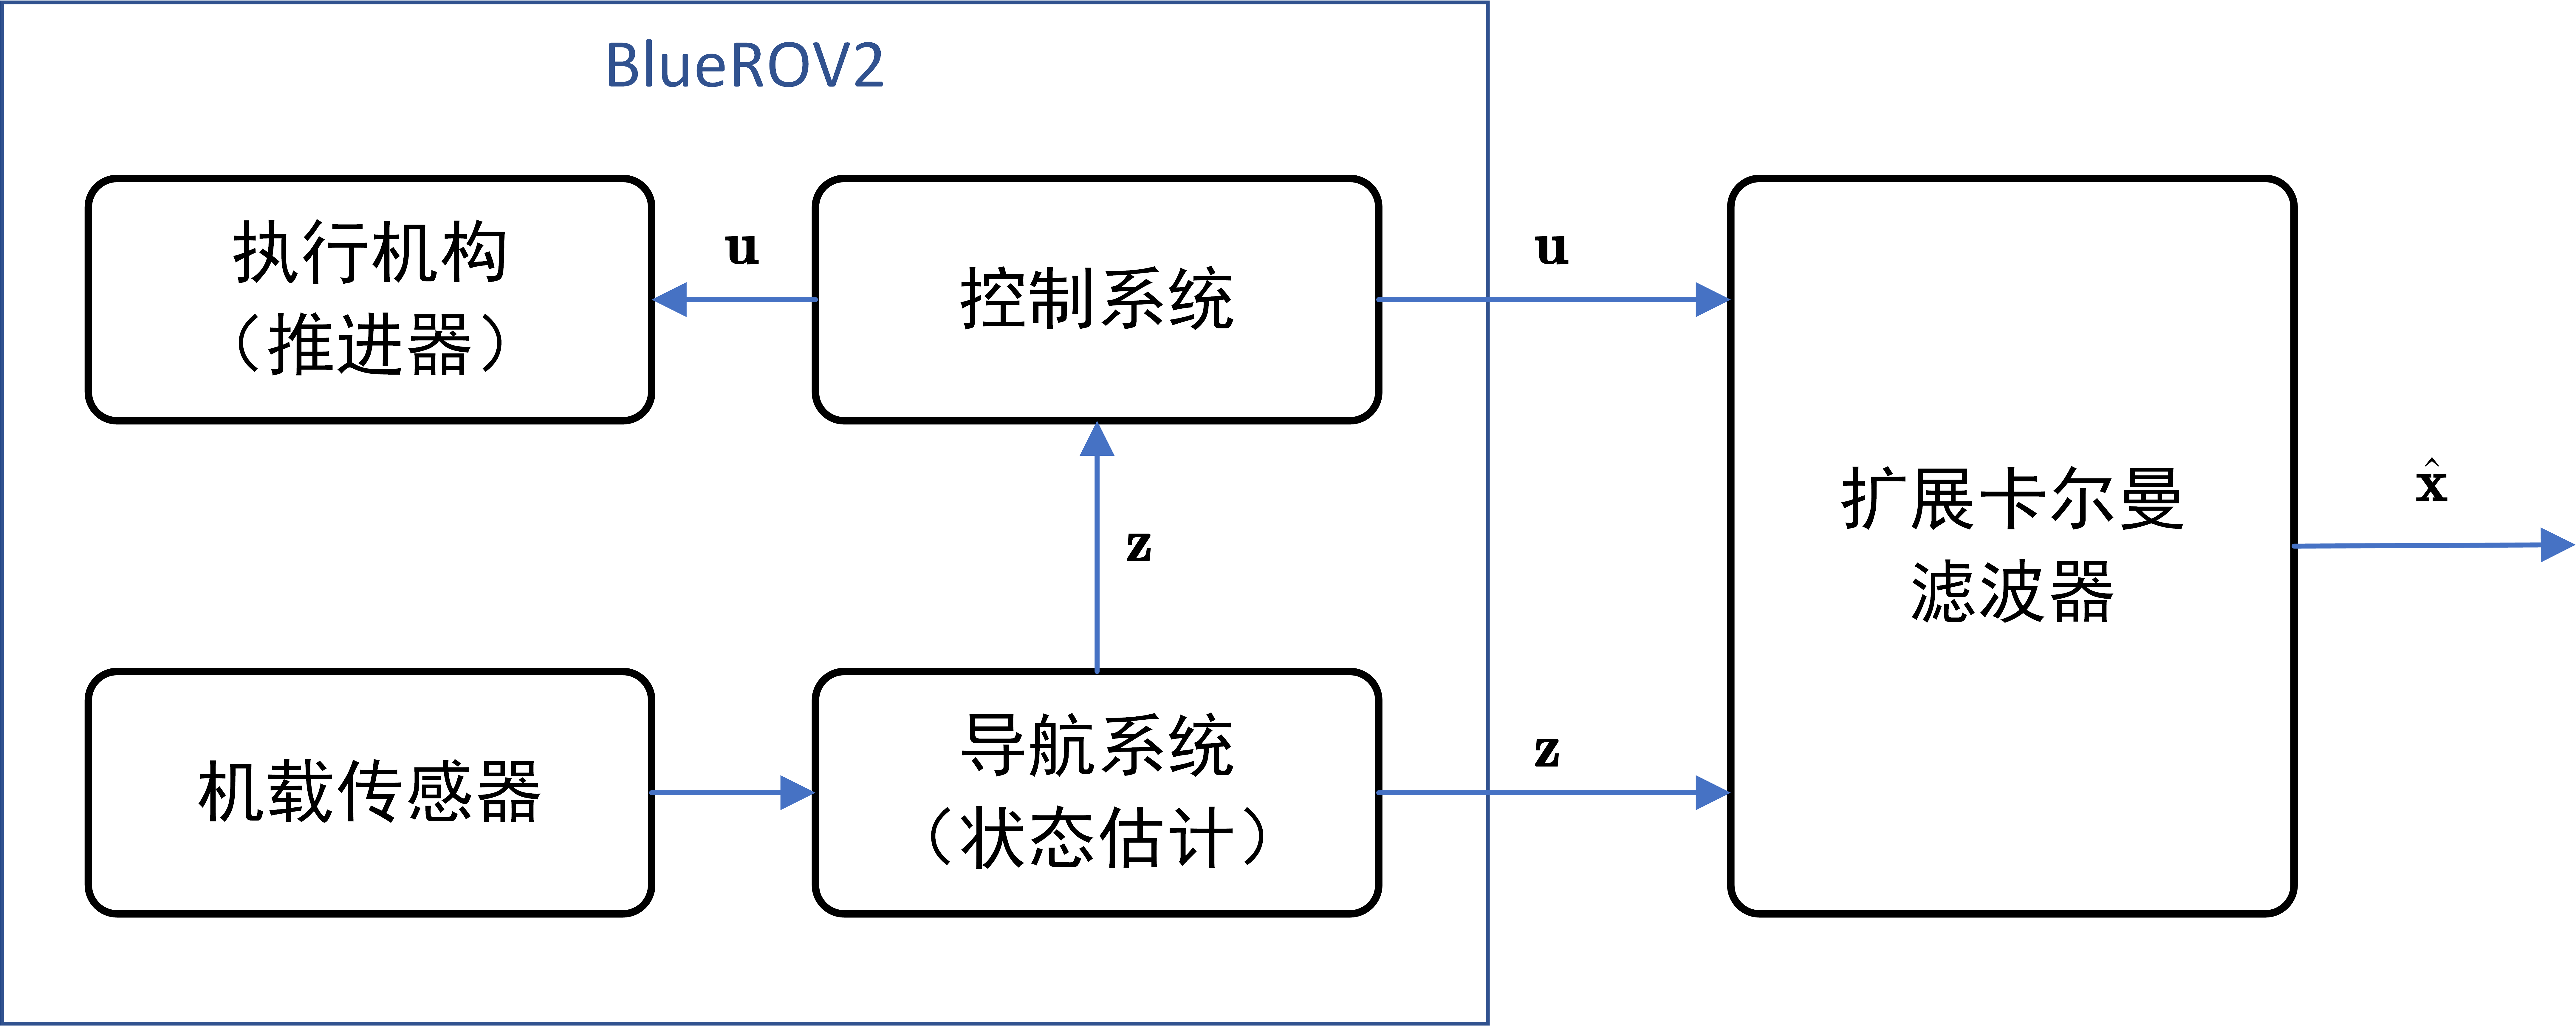
\includegraphics[width=0.7\linewidth]{images/chapter3/卡尔曼滤波辨识流程图.png}
    \caption{扩展卡尔曼滤波器辨识动力学参数流程图}
    \label{f.EKF_ident_frame}
\end{figure}

控制系统内采用传统的PID控制方法,根据预设好的轨迹坐标,设计三个PID控制器分别对水下机器人高度、位置和姿态进行控制,通过PID控制输出BlueROV2导航所需升力、横滚力矩、俯仰力矩、偏航力矩,最后由推力分配矩阵得到各个电机转速的控制信号$\symbf{u}$。PID控制方程为:
\begin{equation}
    u = K_p(x_c-x_r)+K_d\frac{\text{d}(x_c-x_r)}{\text{d}t}+K_i\int_{0}^{t}(x_c-x_r)\text{d}t
\end{equation}
其中,$K_p, K_i, K_d$分别是系统的比例控制系数、微分控制系数和积分控制系数,$x_c$为系统当前状态变量,$x_r$为系统预设状态变量。系统在惯性坐标系下的位姿向量为$\symbf{\eta}=[x,y,z,\phi,\theta,\psi]^T$,则各个位姿分量的控制参数如表\ref{t.PID_params}所示。
\begin{table}[htb]
  \centering
  \caption{BlueROV2各位姿分量PID控制参数}
  \label{t.PID_params}
  \begin{tabular}{cccc}
  \hline
位姿分量 & $K_p$ & $K_d$ & $K_i$ \\
\hline
$x$ & 0.9555 & 1.3650 & -0.3000 \\
$y$ & 0.9555 & 1.3650 & -0.3000 \\
$z$ & -7.8000 & -3.9000 & 5.2000 \\
$\phi$ & 1.6800 & 0.3360 & -2.8000 \\
$\theta$ & 1.6800 & 0.3360 & -2.8000 \\
$\psi$ & 3.2700 & 0.6540 & -5.4500 \\
\hline
\end{tabular}
\end{table}
导航系统中结合了BlueROV2的动力学方程,通过传感器数据测量系统当前状态变量,根据控制输入变量与当前状态测量下一时刻的系统状态。为准确模拟传感器测量误差,本文根据各个传感器测量噪声特点加入噪声以模拟真实的测量环境。扩展卡尔曼滤波器中,根据上述算法更新增广状态向量$\hat{\symbf{x}}$向量,以此得到BlueROV2的动力学模型参数。

扩展卡尔曼滤波器中,需要调增超参数$Q_k$与$R_k$的值,使得卡尔曼滤波器能够较好地模拟实际测量噪声,以此便于模型参数的辨识,通过测试,本文设定卡尔曼滤波器增广状态向量对应的噪声协方差如表所示,其中$P_{ini}$表示增广状态向量的初始协方差,该值会在后续迭代过程中发生改变。

\begin{table}[htb]
  \centering
  \caption{仿真中使用的EKF参数值}
  \label{t.PID_params}
  \zihao{6}
  \begin{tabular}{ccccccccccccc}
  \hline
状态分量 & $x$ & $y$ & $z$ & $\phi$ & $\theta$ & $\psi$ & $u$ & $v$ & $w$ & $p$ & $q$ & $r$ \\
\hline
$P_{ini}$ & 1 & 1 & 1 & 0.1 & 0.1 & 0.1 & 0.1 & 0.1 & 0.1 & 0.1 & 0.1 & 0.1  \\
$Q$ & 0.1 & 0.1 & 0.1 & 0.1 & 0.1 & 0.1 & 0.1 & 0.1 & 0.1 & 0.1 & 0.1 & 0.1  \\
$R$ & 0.01 & 0.01 & 0.01 & 0.0025 & 0.0025 & 0.0025 & 0.0025 & 0.0025 & 0.0025 & 0.0025 & 0.0025 & 0.0025 \\
\hline
\hline
状态分量 & $X_u$ & $Y_v$ & $Z_w$ & $K_p$ & $M_q$ & $N_r$ & $X_{\dot{u}}$ & $Y_{\dot{v}}$ & $Z_{\dot{w}}$ & $K_{\dot{p}}$ & $M_{\dot{q}}$ & $N_{\dot{r}}$ \\
\hline
$P_{ini}$ & 1 & 1 & 1 & 0.1 & 0.1 & 0.1 & 0.1 & 0.1 & 0.1 & 0.1 & 0.1 & 0.1  \\
$Q$ & 0.1 & 0.1 & 0.1 & 0.1 & 0.1 & 0.1 & 0.1 & 0.1 & 0.1 & 0.1 & 0.1 & 0.1  \\
$R$ & - & - & - & - & - & - & - & - & - & - & - & - \\
\hline
\end{tabular}
\end{table}

\subsection{扩展卡尔曼滤波器辨识结果}

通过仿真,本文对于BlueROV2的附加质量系数、一阶阻尼系数进行辨识,辨识的结果分别如图\ref{f.added_mass_ident}和图\ref{f.damping_ident}所示,通过扩展卡尔曼滤波器矩阵辨识,增广状态向量曲线最后收敛至辨识值,辨识值如表\ref{t.ident_results}所示。通过分析增广状态向量收敛曲线,可以发现与附加质量系数相比,一些阻尼系数,主要是 $Y_v$, $K_p$, $N_r$,在辨识初期表现出更明显的振荡行为,之后才逐渐稳定。这表明这些参数的辨识过程可能对初始扰动或模型耦合更为敏感,或者EKF的调整使得它们需要更长时间来抑制瞬态,而$X_u$, $Z_w$, $M_q$ 的收敛过程相对平滑,振荡不明显。

\begin{figure}[hbt]
    \centering
    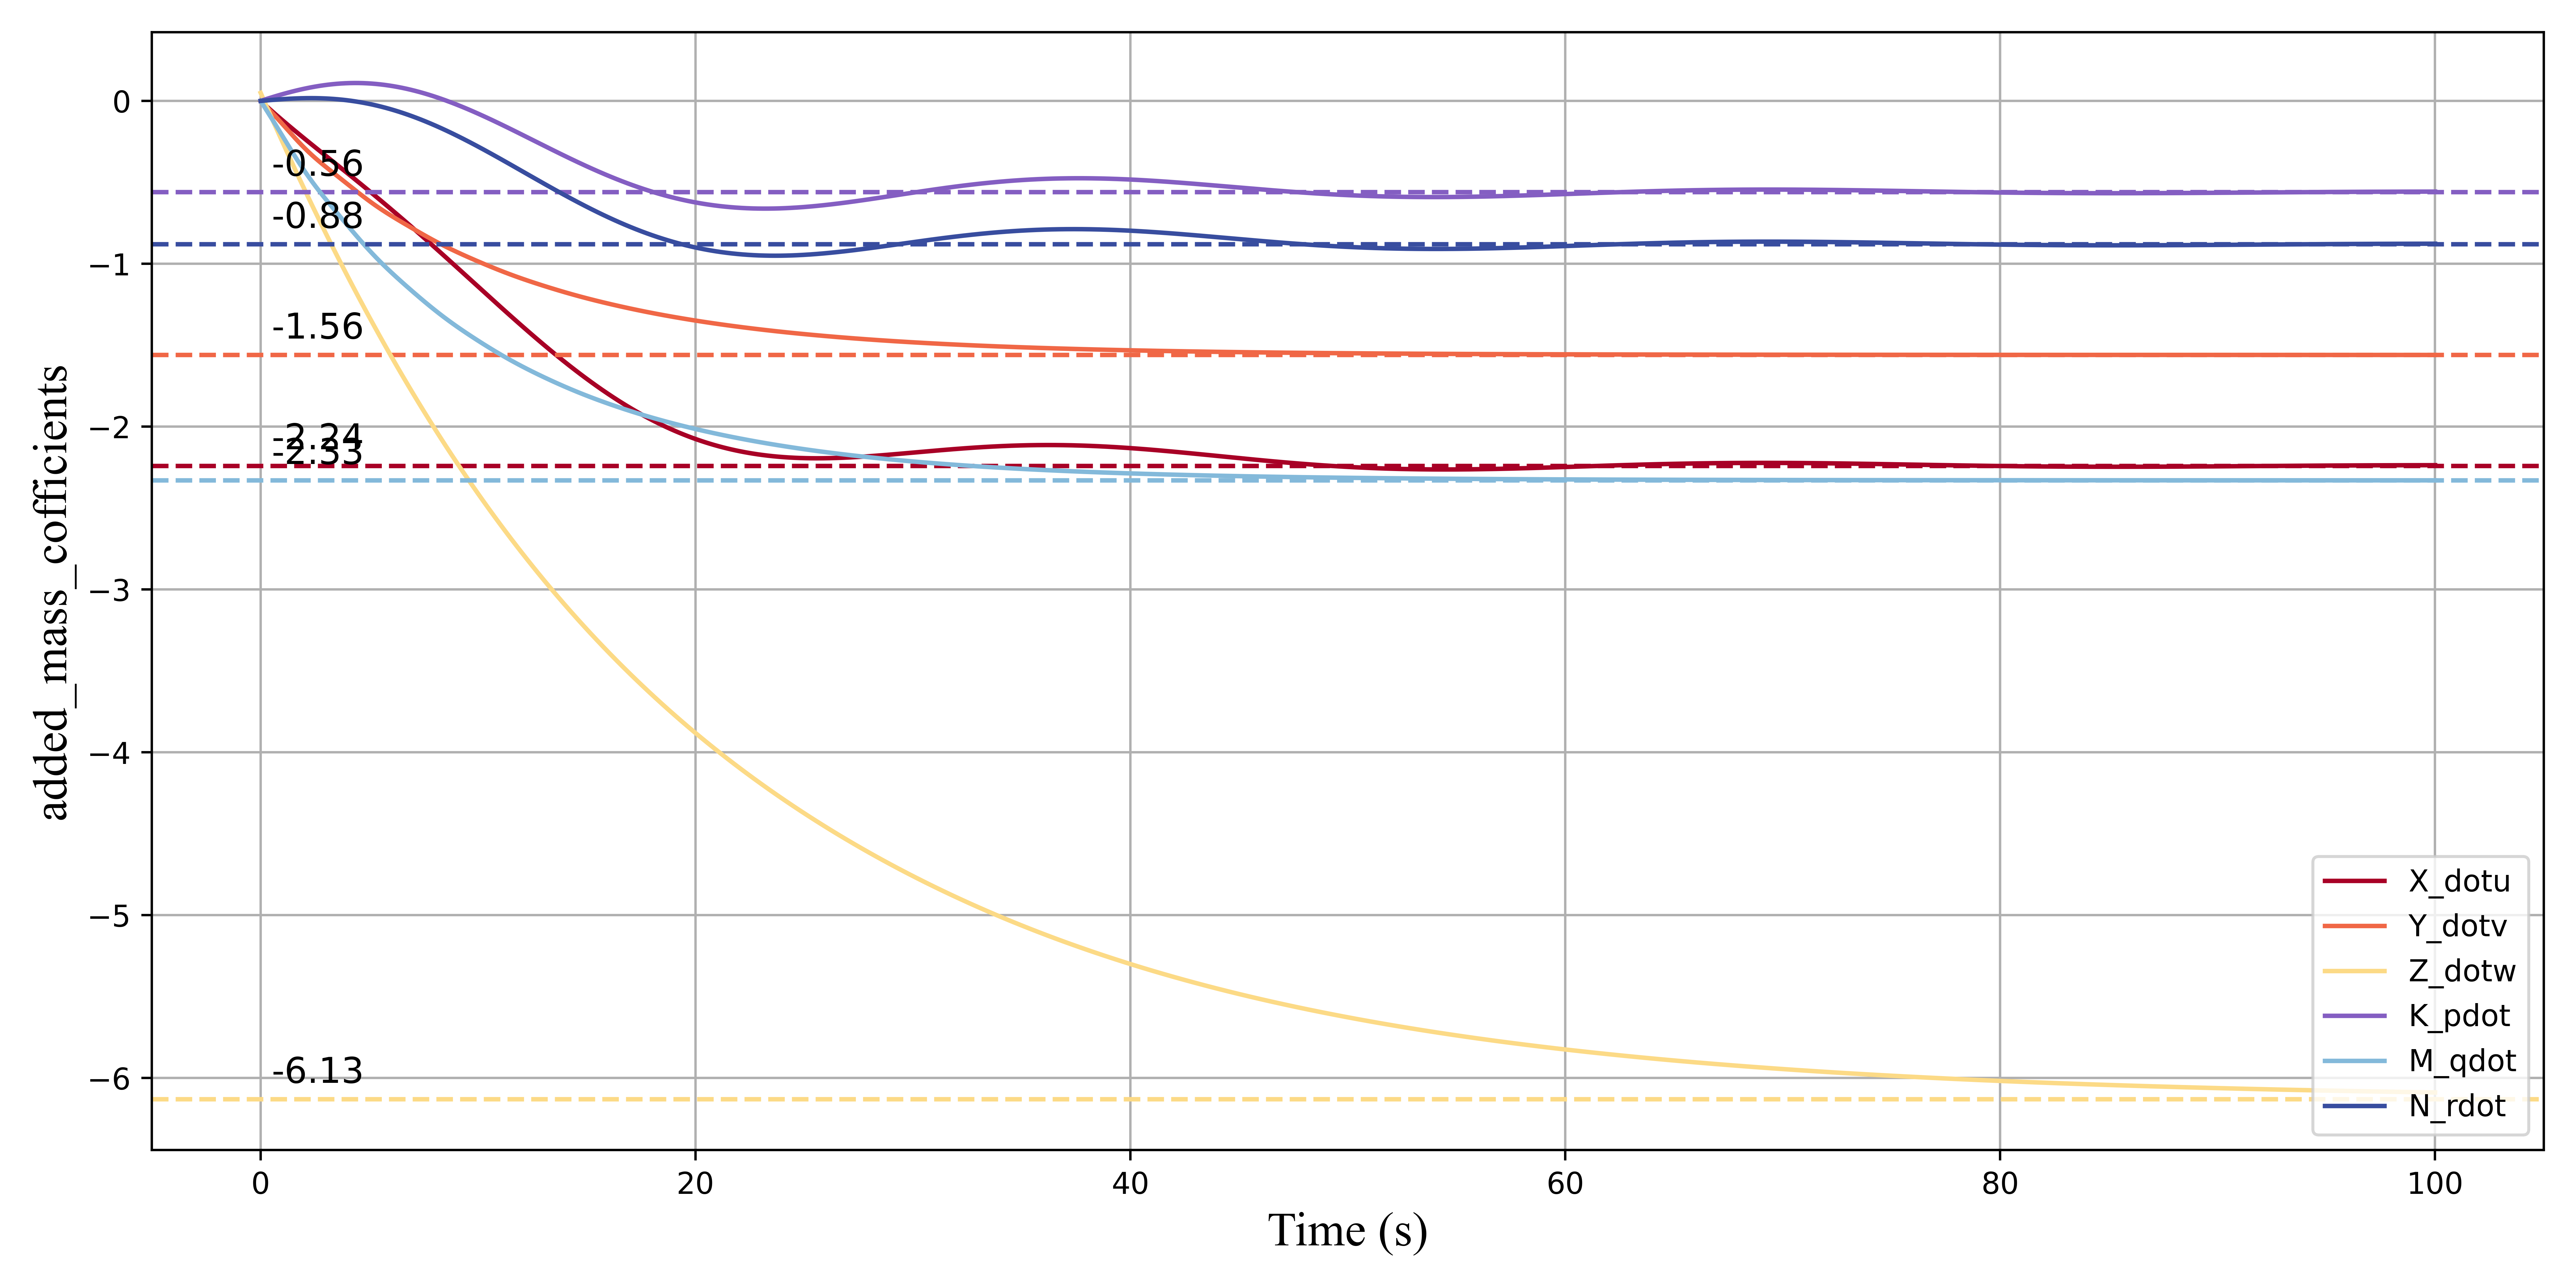
\includegraphics[width=0.8\linewidth]{images/chapter3/附加质量辨识结果.png}
    \caption{BlueROV2附加质量系数辨识}
    \label{f.added_mass_ident}
\end{figure}

\begin{figure}[hbt]
    \centering
    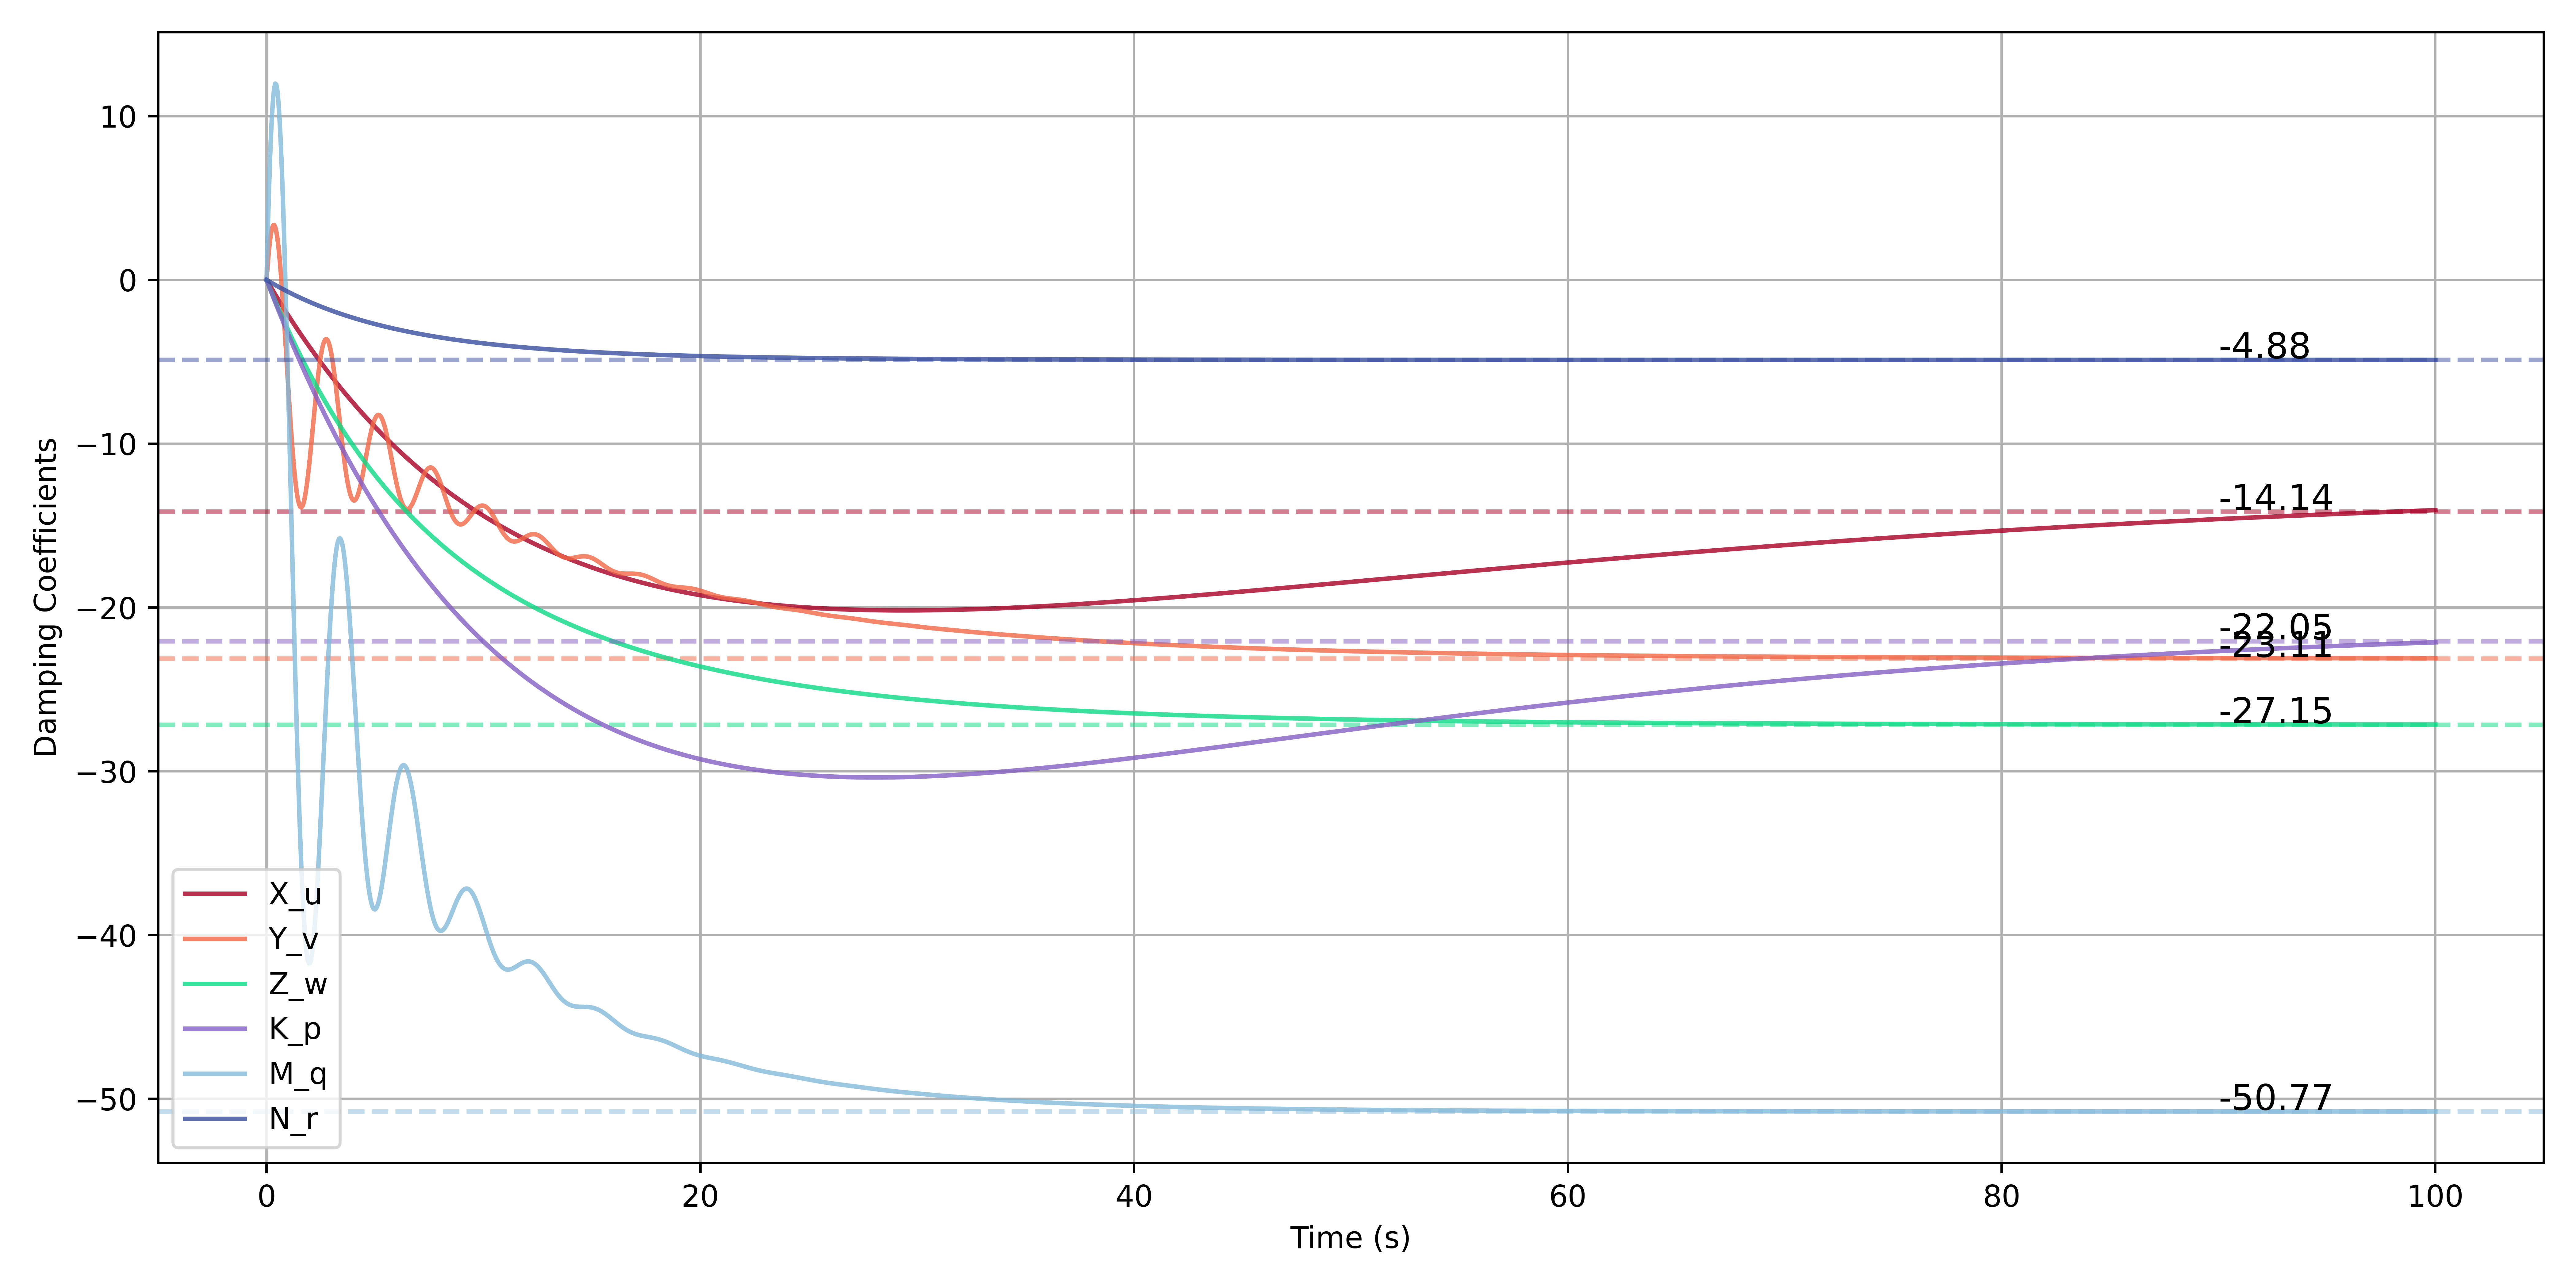
\includegraphics[width=0.8\linewidth]{images/chapter3/阻尼系数辨识结果.png}
    \caption{BlueROV2一阶阻尼系数辨识}
    \label{f.damping_ident}
\end{figure}

\begin{table}[htb]
  \centering
  \caption{扩展卡尔曼滤波器辨识系数结果}
  \label{t.ident_results}
  \begin{tabular}{ccccccc}
  \hline
符号 & $X_{\dot{u}}$ & $Y_{\dot{v}}$ & $Z_{\dot{w}}$ & $K_{\dot{p}}$ & $M_{\dot{q}}$ & $N_{\dot{r}}$ \\
\hline
辨识值  & -2.24  & -1.56 & -6.13  & -0.56 & -2.33 & -0.88   \\
\hline
\hline
符号 & $X_u$ & $Y_v$ & $Z_w$ & $K_p$ & $M_q$ & $N_r$ \\
\hline
辨识值  & -14.14 & -23.11  & -27.15 & -22.05  & -50.77 & -4.88 \\
\hline
\end{tabular}
\end{table}

通过上述仿真结构,本文提取BlueROV2状态向量在已辨识系数下的表现。图\ref{f.EKF_position}和图\ref{f.EKF_vel}分别展示了广义位姿向量$[p_n,p_e,p_d,\phi, \theta, \psi]^T$和广义速度向量$[u,v,w,p,q,r]^T$的实际值和测量值的时间序列曲线,其中实际值为蓝色曲线,表示在控制输入和真实水动力系数下BlueROV2的运动曲线,测量值表示在控制输入和辨识水动力系数下BlueROV2的运动曲线,此外,由于控制输入是对BlueROV2深度坐标和姿态信息$[\phi, \theta,\psi]^T$的控制,其中的绿色曲线表示对应的控制信号。

通过信号对比可以发现,辨识出的系统在深度方向上的速度$w$表现较差,测量值存在噪音明显,与实际值不符,而系统在姿态控制上符合良好,表明该系统能够有效地处理BlueROV2系统的姿态控制,而在位置坐标控制上表现较弱。

\begin{figure}[hbt]
    \centering
    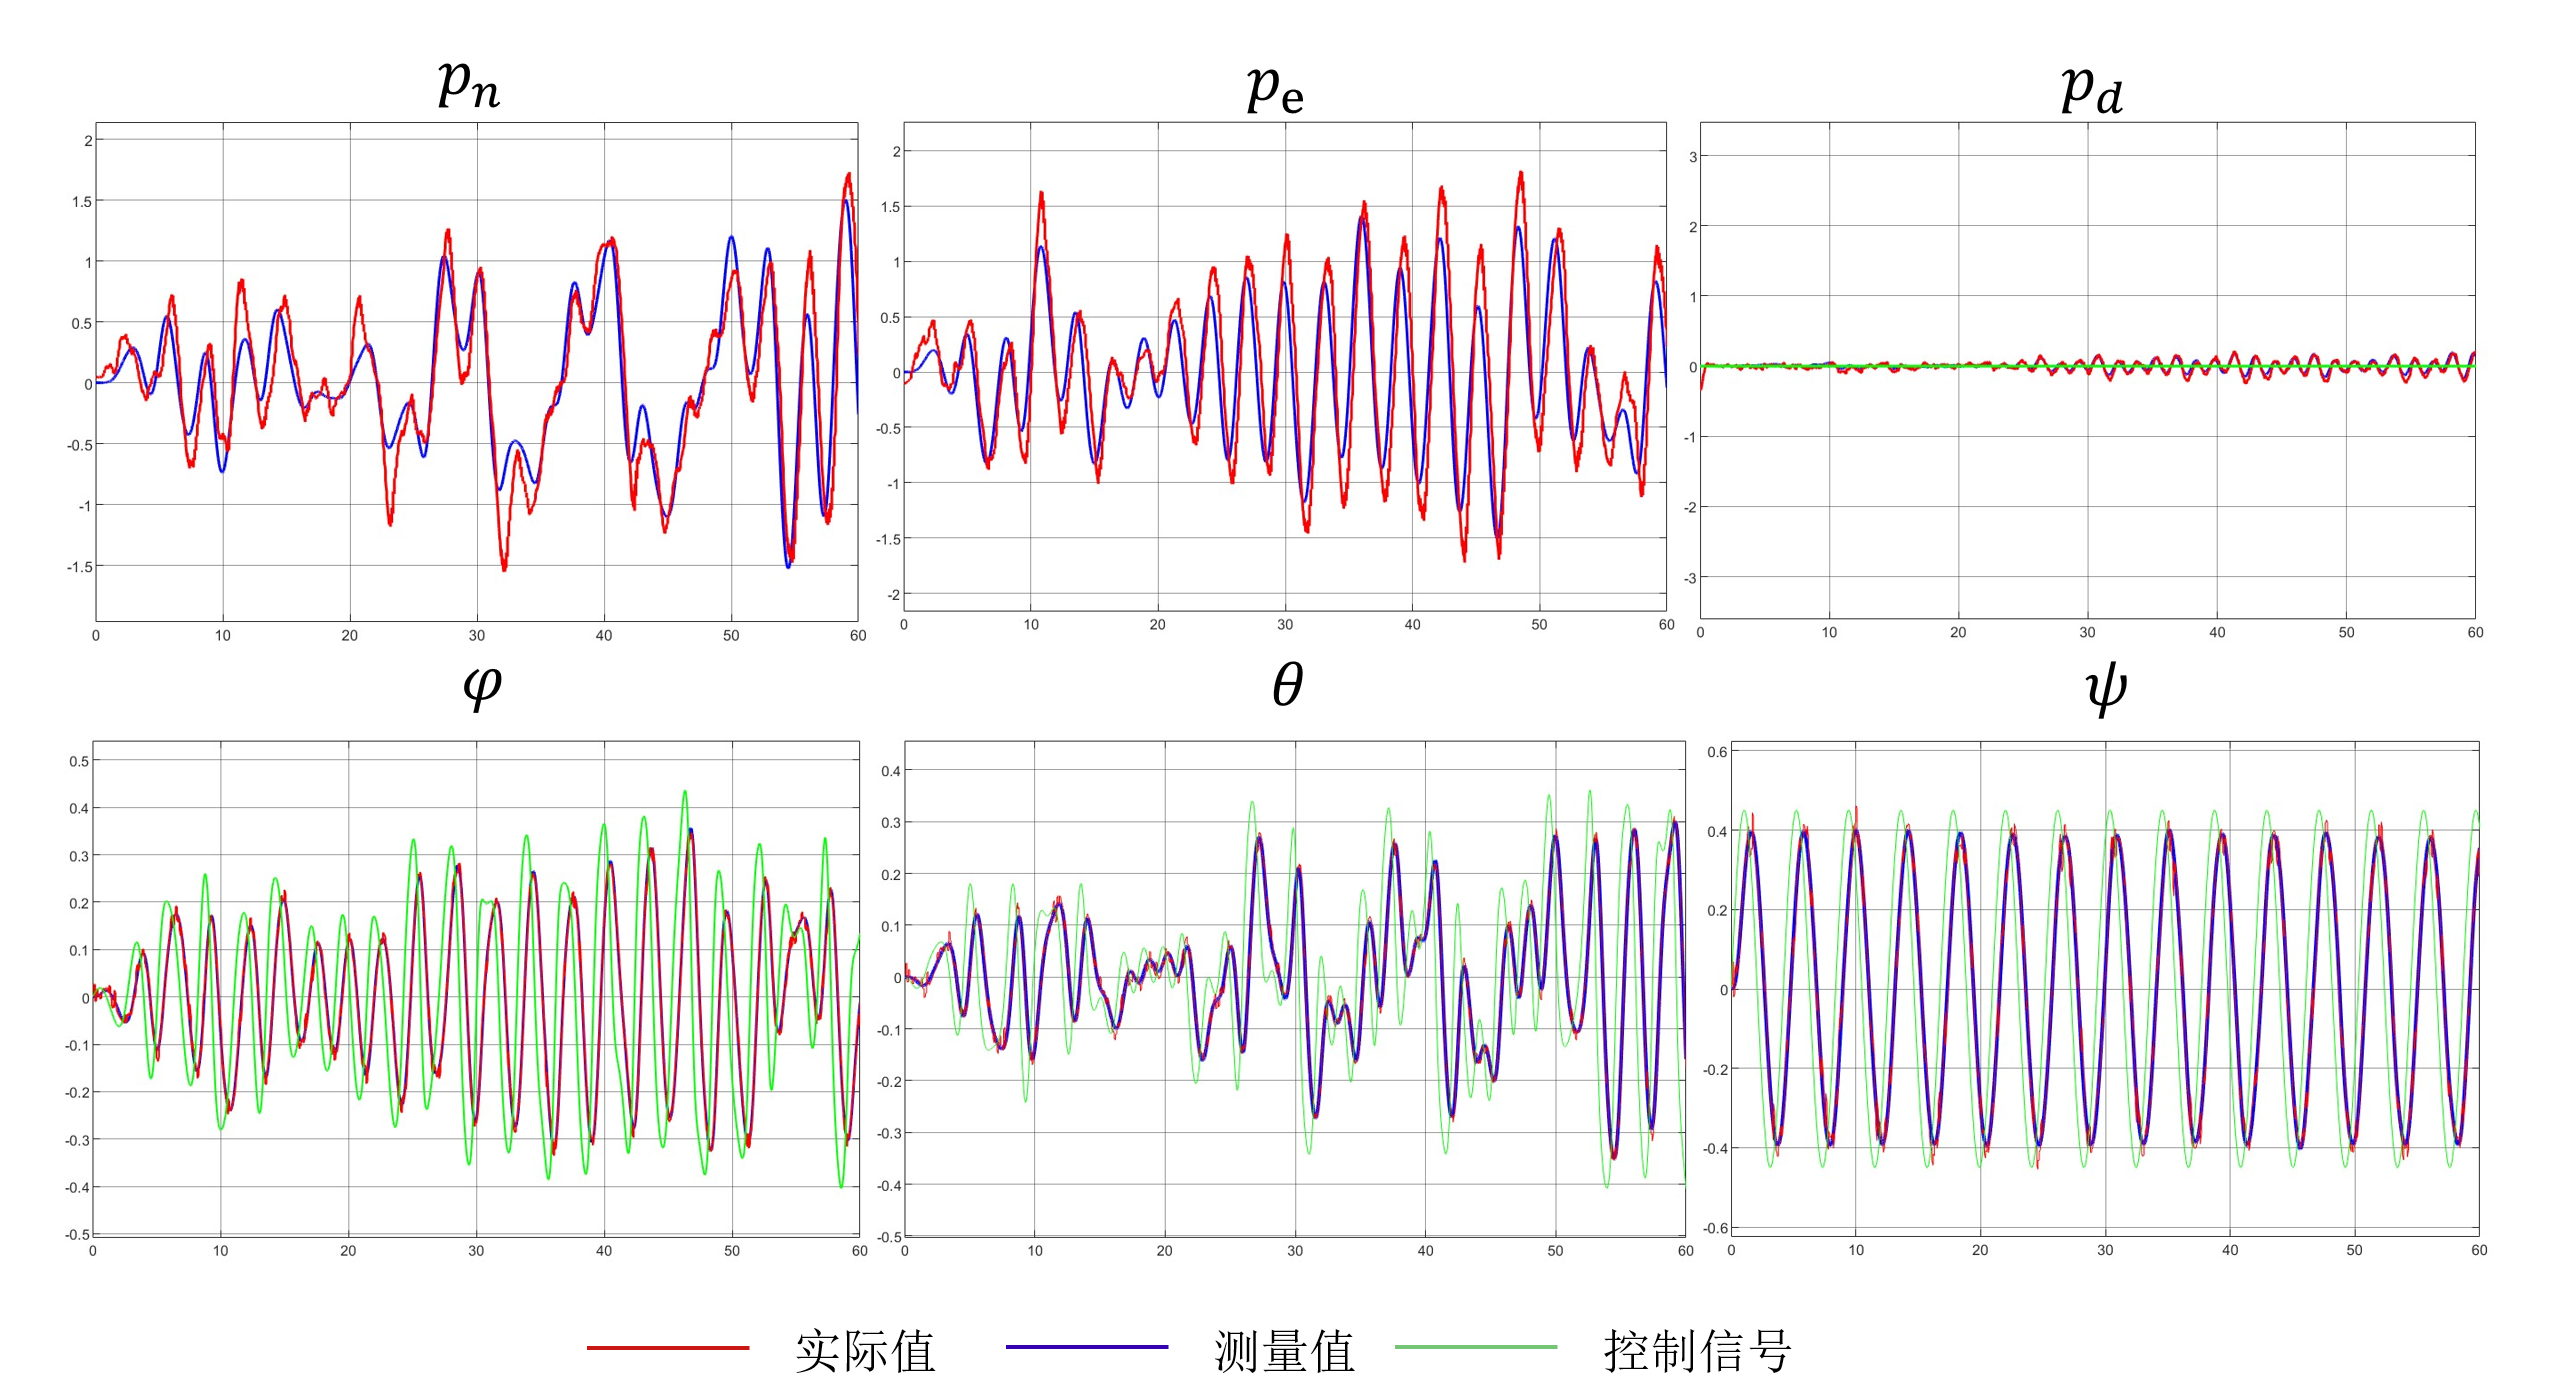
\includegraphics[width=0.8\linewidth]{images/chapter3/EKF_position.png}
    \caption{BlueROV2广义位姿向量辨识效果}
    \label{f.EKF_position}
\end{figure}
\begin{figure}[hbt]
    \centering
    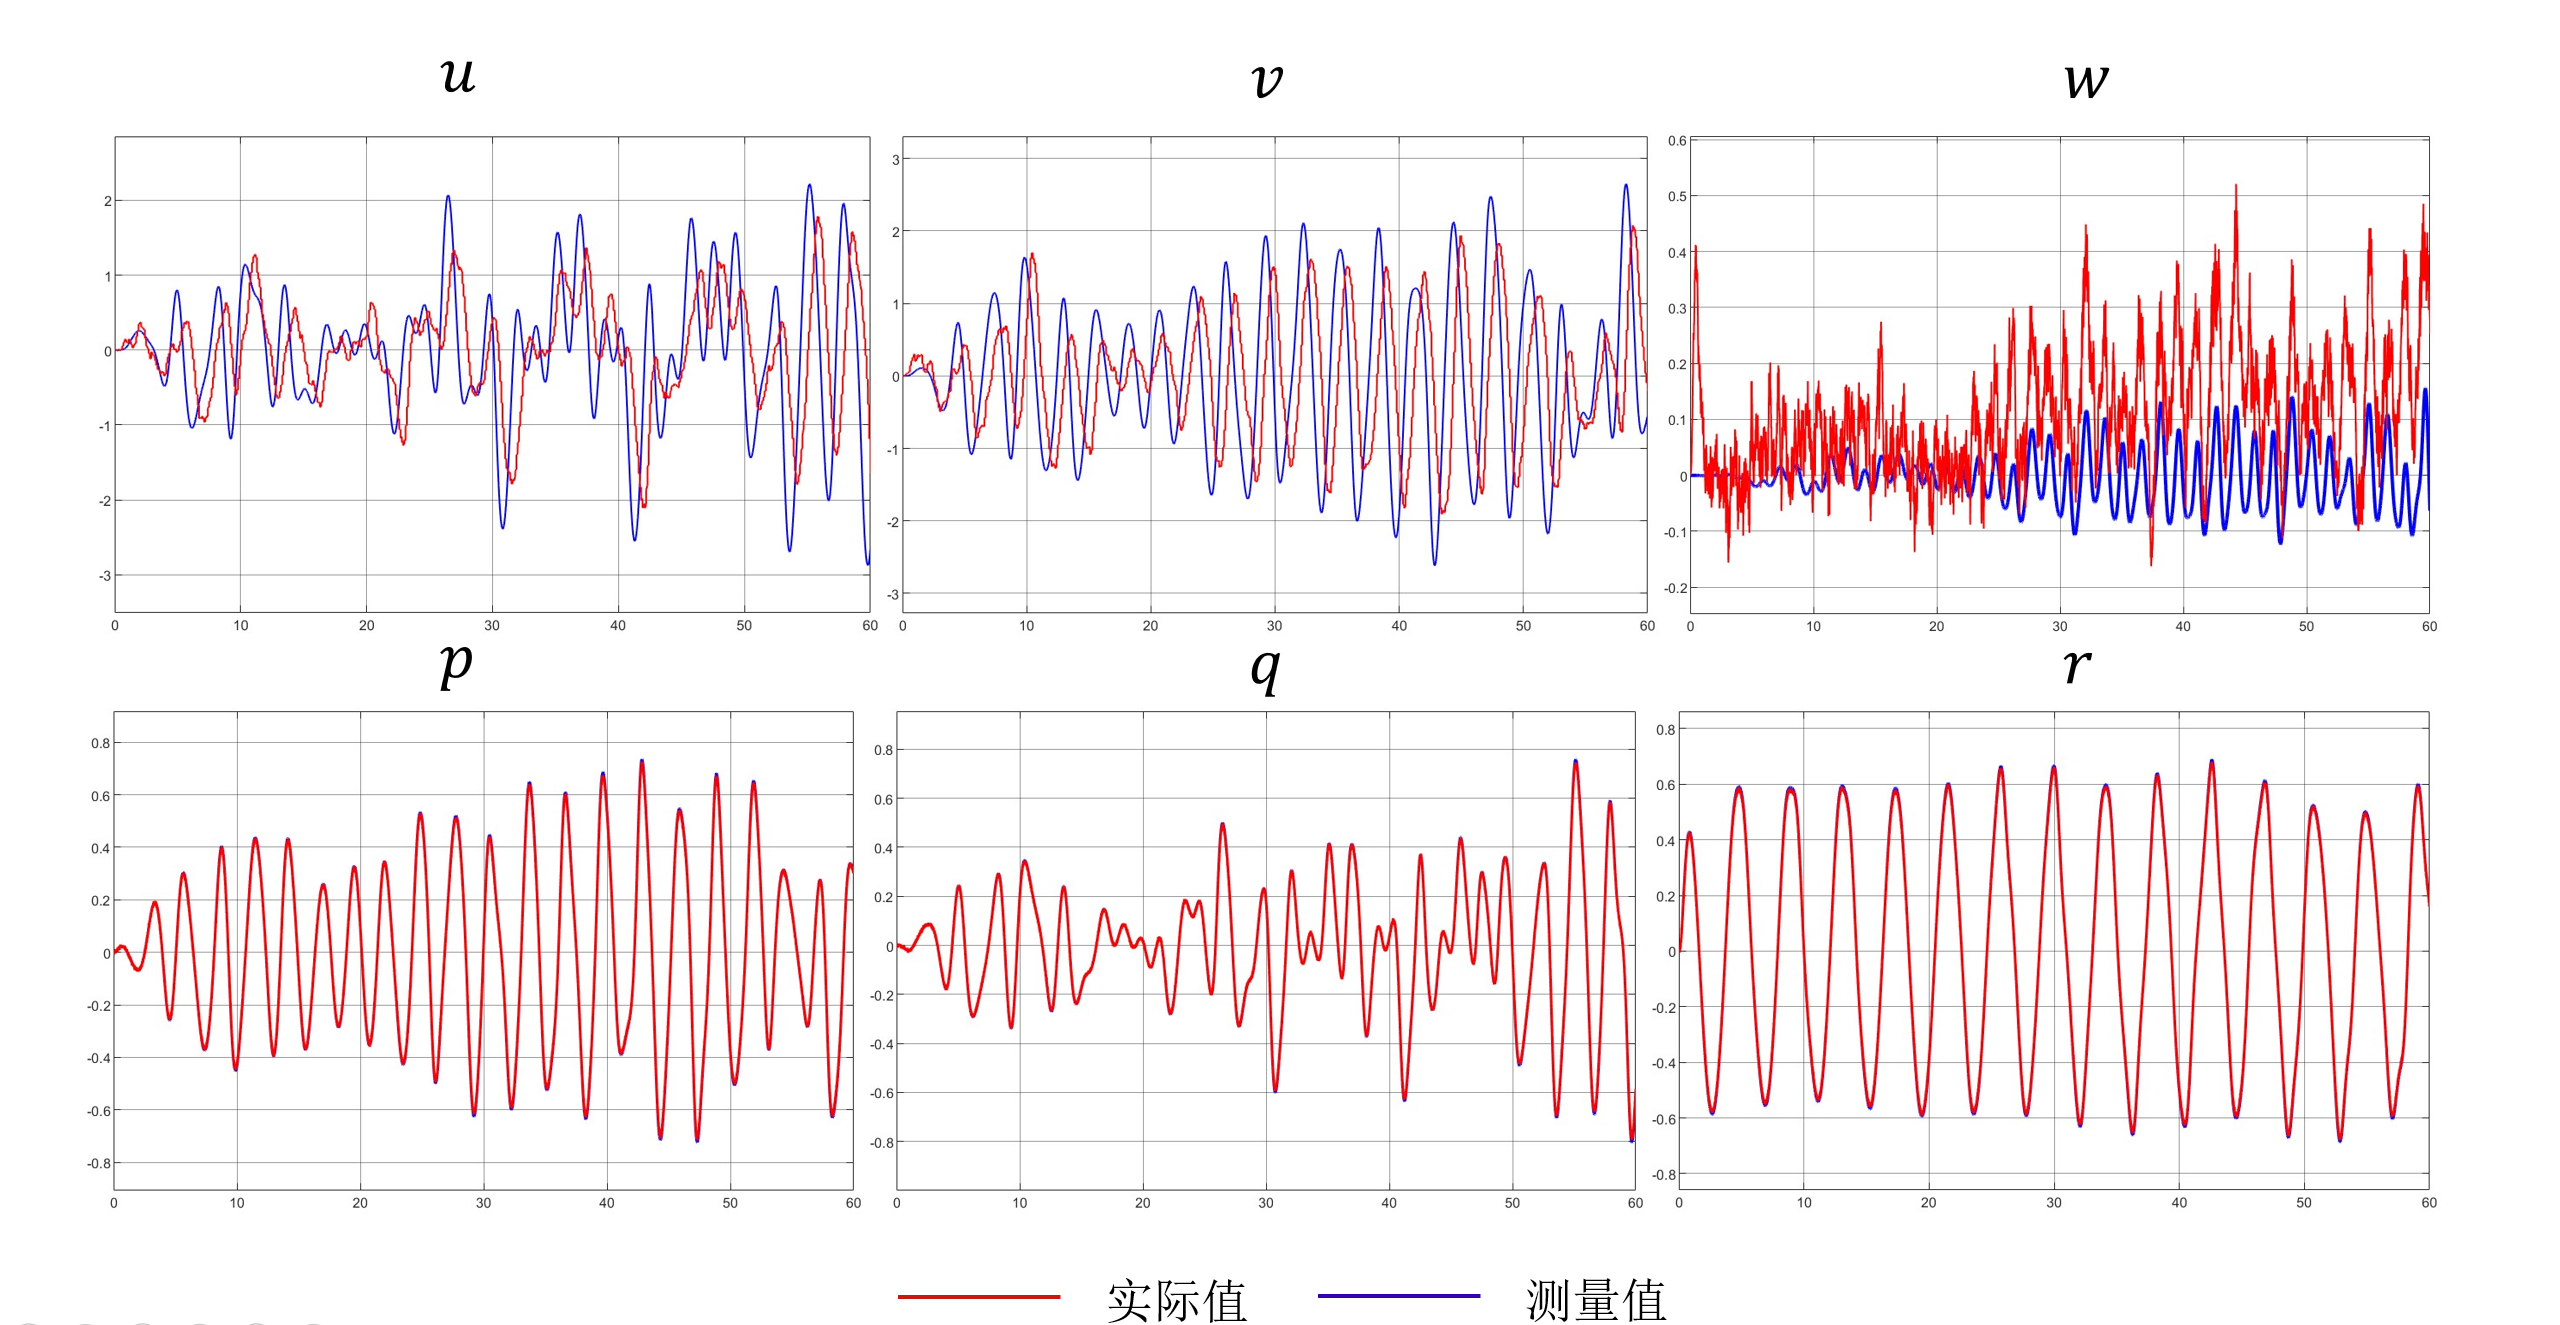
\includegraphics[width=0.8\linewidth]{images/chapter3/EKF_vel.png}
    \caption{BlueROV2广义速度向量辨识效果}
    \label{f.EKF_vel}
\end{figure}

\section{本章小结}

本章节在前一章节完成BlueROV2动力学建模的基础上,通过最小二乘法和扩展卡尔曼滤波方法对BlueROV2动力学模型未知参数进行辨识。考虑到需要辨识的有18个参数,六自由度的动力学方程与参数个数不兼容,故将运动曲线解耦为水平面运动模型与竖直面运动模型分别分析,辨识出水动力系数;而在扩展卡尔曼滤波方法中,通过建立MATLAB/Simulink仿真结构,模拟机载传感器测量噪声和控制信号,建立增广状态向量,完成了动力学参数的辨识,并且将实际值和测量值曲线进行了比较,得到卡尔曼滤波方法的辨识特性。

\newpage